\begin{minipage}{0.75\linewidth}
\begin{figure}[h]
    \centering
    \begin{adjustbox}{max width=1.0\linewidth, keepaspectratio}
        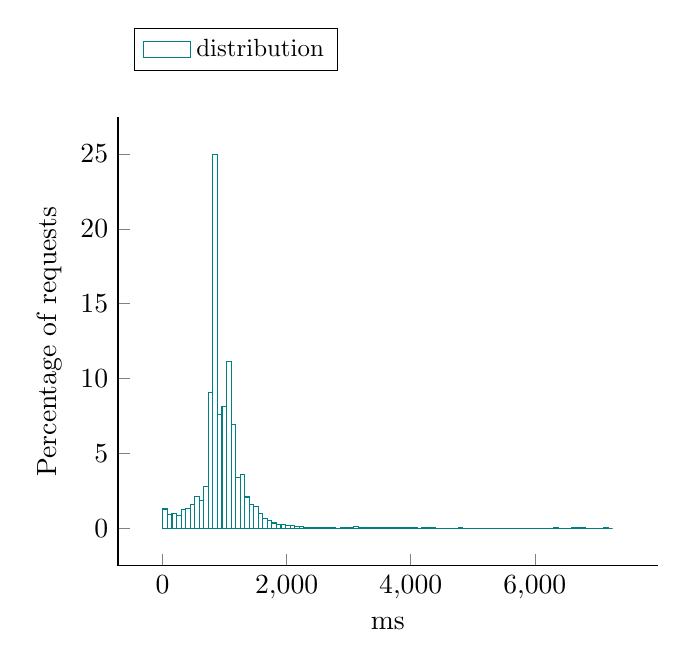
\begin{tikzpicture}
            \begin{axis}[ylabel = Percentage of requests, 
xlabel = ms, 
legend style = {nodes={scale=0.9, transform shape}, at={(0.03,1.2)}, anchor=north west, draw=black, fill=white, align=left, legend columns=3},
area style, mark size = 0pt,
 cycle list name = exotic,
  axis lines* = left]
		\addplot +[ybar interval] coordinates {
			 (5, 1.2872)
			 (78.23, 0.926784)
			 (151.46, 0.998867)
			 (224.69, 0.875296)
			 (297.92, 1.2666)
			 (371.15, 1.2975)
			 (444.38, 1.56524)
			 (517.61, 2.12131)
			 (590.84, 1.83297)
			 (664.07, 2.77005)
			 (737.3, 9.07219)
			 (810.53, 24.9511)
			 (883.76, 7.58933)
			 (956.99, 8.1351)
			 (1030.22, 11.1111)
			 (1103.45, 6.93029)
			 (1176.68, 3.38791)
			 (1249.91, 3.59386)
			 (1323.14, 2.09041)
			 (1396.37, 1.58583)
			 (1469.6, 1.44166)
			 (1542.83, 0.98857)
			 (1616.06, 0.648749)
			 (1689.29, 0.494285)
			 (1762.52, 0.350118)
			 (1835.75, 0.25744)
			 (1908.98, 0.226547)
			 (1982.21, 0.195654)
			 (2055.44, 0.175059)
			 (2128.67, 0.123571)
			 (2201.9, 0.0926784)
			 (2275.13, 0.0720832)
			 (2348.36, 0.0411904)
			 (2421.59, 0.0823808)
			 (2494.82, 0.051488)
			 (2568.05, 0.0308928)
			 (2641.28, 0.0411904)
			 (2714.51, 0.0720832)
			 (2787.74, 0.0102976)
			 (2860.97, 0.0720832)
			 (2934.2, 0.051488)
			 (3007.43, 0.0308928)
			 (3080.66, 0.102976)
			 (3153.89, 0.0205952)
			 (3227.12, 0.0411904)
			 (3300.35, 0.051488)
			 (3373.58, 0.0411904)
			 (3446.81, 0.0308928)
			 (3520.04, 0.051488)
			 (3593.27, 0.0720832)
			 (3666.5, 0.0617856)
			 (3739.73, 0.0411904)
			 (3812.96, 0.0308928)
			 (3886.19, 0.0617856)
			 (3959.42, 0.0823808)
			 (4032.65, 0.0205952)
			 (4105.88, 0)
			 (4179.11, 0.0308928)
			 (4252.34, 0.0205952)
			 (4325.57, 0.0308928)
			 (4398.8, 0)
			 (4472.03, 0.0102976)
			 (4545.26, 0)
			 (4618.49, 0)
			 (4691.72, 0)
			 (4764.95, 0.0205952)
			 (4838.18, 0)
			 (4911.41, 0.0102976)
			 (4984.64, 0.0102976)
			 (5057.87, 0)
			 (5131.1, 0.0102976)
			 (5204.33, 0)
			 (5277.56, 0.0102976)
			 (5350.79, 0)
			 (5424.02, 0)
			 (5497.25, 0)
			 (5570.48, 0)
			 (5643.71, 0.0102976)
			 (5716.94, 0)
			 (5790.17, 0)
			 (5863.4, 0)
			 (5936.63, 0)
			 (6009.86, 0.0102976)
			 (6083.09, 0)
			 (6156.32, 0.0102976)
			 (6229.55, 0.0102976)
			 (6302.78, 0.0205952)
			 (6376.01, 0.0102976)
			 (6449.24, 0.0102976)
			 (6522.47, 0.0102976)
			 (6595.7, 0.0205952)
			 (6668.93, 0.0205952)
			 (6742.16, 0.0205952)
			 (6815.39, 0)
			 (6888.62, 0)
			 (6961.85, 0)
			 (7035.08, 0)
			 (7108.31, 0.0308928)
			 (7181.54, 0)
			 (7254.77, 0)
		};
\addlegendentry{distribution};
           \end{axis}
      \end{tikzpicture}
  \end{adjustbox}
  \caption{Response time distribution - req = ReadUser-0}
\end{figure}
\end{minipage}\hfill\begin{minipage}{0.18\linewidth}
\begin{table}[h]
\begin{tabular}{|cc|}
\hline
\textbf{} & \textbf{ms}\\ \hline
 \Xhline{0.005\arrayrulewidth}
min & 5\\
 \Xhline{0.005\arrayrulewidth}
max & 7328\\
 \Xhline{0.005\arrayrulewidth}
mean & 978\\
 \Xhline{0.005\arrayrulewidth}
std & 497\\
\hline
\hline
 \Xhline{0.005\arrayrulewidth}
25th & 814\\
 \Xhline{0.005\arrayrulewidth}
50th & 890\\
 \Xhline{0.005\arrayrulewidth}
75th & 1096\\
 \Xhline{0.005\arrayrulewidth}
80th & 1141\\
 \Xhline{0.005\arrayrulewidth}
85th & 1229\\
 \Xhline{0.005\arrayrulewidth}
90th & 1331\\
 \Xhline{0.005\arrayrulewidth}
95th & 1556\\
 \Xhline{0.005\arrayrulewidth}
99th & 3131\\
\hline
\end{tabular}
\caption{Response time}
\end{table}
\end{minipage}\hfill